\chapter{Black Hole Horizons, Acceleration Horizons, and Evaporation}

These notes follow Leonard Susskind's third lecture in the supplementary 2011 ``Winter Topics in String Theory'' track, curated by LazyingArt LLC. The lecture unfolds in two distinct movements. First, Susskind wants to make good on a physical claim from the previous meeting: the horizon of a sufficiently large black hole should feel locally like empty flat space, even though the Schwarzschild metric seems to misbehave at \(r=2MG\). Second, once that local geometry is under control, he turns back to black-hole thermodynamics and asks what temperature, negative specific heat, and evaporation are trying to tell us about the underlying microscopic theory.

\section{Why the Horizon Should Be Boring}

Susskind opens by stating the conclusion he wants the mathematics to explain. If a black hole is very large, then an observer who falls through the horizon should find nothing dramatic there. Locally, the geometry should look exactly, or almost exactly, like empty Minkowski space. The horizon is therefore supposed to be physically boring.

What makes this claim nontrivial is the familiar Schwarzschild metric. In Schwarzschild coordinates, one coefficient vanishes at \(r=2MG\) and another diverges there. The lecture begins by sharpening that tension rather than hiding it. The question is not whether the metric looks singular in these coordinates; it plainly does. The question is whether that behavior signals real physics or only a bad coordinate choice.

\section{Metric Convention and the Schwarzschild Starting Point}

Susskind next resets notation. Earlier lectures used \(d\tau^2\), positive on timelike intervals. Here he flips the overall sign and works with \(ds^2\), which he describes as a ``proper distance squared'' convention. Nothing essential changes, but the formulas now appear in the form he prefers to manipulate on the blackboard. Throughout these notes I write \(M\) and \(G\), although the spoken lecture often says \(m\) and \(g\).

\begin{figure}[h]
\centering

\includegraphics[width=0.54\textwidth]{lecture_03_figure_02.png}
\caption{Board evidence for the sign-convention shift and the beginning of the Schwarzschild rewrite. The top line is a transitional reference line; the transcript controls the polished metric written below.}
\end{figure}

\begin{remark}
The visible board line
\[
ds^2 = dt^2 - dx^2
\]
should be read as a transitional flat-space reference during the sign change, not as the final governing convention for the lecture's black-hole formulas.
\end{remark}

Suppressing the angular part exactly as Susskind does, the Schwarzschild metric is written as
\begin{equation}
ds^2 = -\left(1-\frac{2MG}{r}\right)dt^2 + \frac{dr^2}{1-\frac{2MG}{r}} + \cdots .
\end{equation}
The omitted term is the angular piece \(r^2 d\Omega_2^2\), which plays no role in the near-horizon derivation. Far from the hole, where \(r \gg 2MG\), one has
\begin{equation}
ds^2 \approx -dt^2 + dr^2 + \cdots ,
\end{equation}
so the radial-time geometry is just the flat metric.

The trouble begins near \(r=2MG\). There the coefficient of \(dt^2\) goes to zero, while the coefficient of \(dr^2\) becomes large. Susskind's point is that this is only the beginning of the story. Before touching the black hole directly, he moves ``over here'' on the board and reviews a pair of coordinate systems whose whole purpose is to teach the audience not to overreact to singular-looking metric coefficients.

\section{A Coordinate Warm-Up: Polar and Hyperbolic Polar Coordinates}

\paragraph{Polar coordinates on the plane.}
On the ordinary Euclidean plane the metric is
\begin{equation}
ds^2 = dx^2 + dy^2.
\end{equation}
Now introduce polar coordinates,
\begin{equation}
x=\rho\cos\theta,
\qquad
y=\rho\sin\theta.
\end{equation}
A small displacement has one component \(d\rho\) in the radial direction and one component \(\rho\,d\theta\) in the transverse direction, so the metric becomes
\begin{equation}
ds^2 = d\rho^2 + \rho^2 d\theta^2.
\end{equation}
At \(\rho=0\), the coefficient of \(d\theta^2\) vanishes. But nothing singular happens at the origin. It merely means that changing \(\theta\) at the origin does not move you anywhere. This is the first model of the phenomenon Susskind wants the class to keep in mind.

\paragraph{Hyperbolic polar coordinates in Minkowski space.}
He then replaces the Euclidean plane by \(1+1\)-dimensional Minkowski space,
\begin{equation}
ds^2 = -dt^2 + dx^2.
\end{equation}
Again he introduces a radial variable \(\rho\), but the angular variable is now a hyperbolic angle \(\omega\):
\begin{equation}
x=\rho\cosh\omega,
\qquad
t=\rho\sinh\omega.
\end{equation}
The corresponding identity is no longer \(\cos^2\theta+\sin^2\theta=1\), but
\begin{equation}
\cosh^2\omega-\sinh^2\omega=1.
\end{equation}
One may picture \(\cosh\omega\) and \(\sinh\omega\) by using the unit hyperbola \(x^2-t^2=1\) in exactly the way ordinary sine and cosine are pictured on the unit circle.

Substituting these variables into the flat Minkowski metric gives
\begin{equation}
ds^2 = -\rho^2 d\omega^2 + d\rho^2.
\end{equation}
This is still flat spacetime. Nothing physical has changed. Only the coordinates are different. Susskind explicitly tells the class to remember this formula and even leaves it on the board, because it is the form he wants to recognize later in the near-horizon Schwarzschild geometry.

A useful difference from ordinary polar coordinates is that \(\theta\) is periodic, while \(\omega\) is not. The variable \(\omega\) runs from \(-\infty\) to \(+\infty\), and as \(|\omega|\) becomes large the hyperbola approaches the light cone. In this sense \(\omega\) behaves like a time variable adapted to uniformly accelerated observers.

\section{The Near-Horizon Reduction}

Susskind now returns to the black hole and states the real target of the calculation: the Schwarzschild metric near \(r=2MG\) should reduce to the same hyperbolic-polar form just written for flat space.

The first step is only algebra. Rewrite the radial-time part of the metric as
\begin{align}
ds^2
&= -\left(1-\frac{2MG}{r}\right)dt^2 + \frac{dr^2}{1-\frac{2MG}{r}} \\
&= -\frac{r-2MG}{r}\,dt^2 + \frac{r}{r-2MG}\,dr^2 .
\end{align}
Nothing has been approximated yet.

The approximation enters only after Susskind says that he wants to zoom in on \(r=2MG\). There is one delicate point, and he slows down to emphasize it. Near the horizon, one may replace \(r\) by \(2MG\) where it varies slowly, but one should \emph{not} tamper with \(r-2MG\), because that quantity changes sign across the horizon. With that rule, the metric becomes
\begin{equation}
ds^2 \approx -\frac{r-2MG}{2MG}\,dt^2 + \frac{2MG}{r-2MG}\,dr^2.
\end{equation}
This approximation is not exact, but it becomes arbitrarily accurate as one restricts attention more and more tightly to the neighborhood of \(r=2MG\).

The next move is a change of radial coordinate. Susskind chooses \(\rho\) so that the entire radial term simply becomes \(d\rho^2\):
\begin{equation}
d\rho^2 = \frac{2MG}{r-2MG}\,dr^2.
\end{equation}
Taking square roots gives
\begin{equation}
d\rho = \sqrt{\frac{2MG}{r-2MG}}\,dr,
\end{equation}
and integrating gives
\begin{equation}
\rho = 2\sqrt{2MG}\,\sqrt{r-2MG}.
\end{equation}
Squaring this relation produces the especially useful form
\begin{equation}
\rho^2 = 8MG(r-2MG),
\qquad
r-2MG = \frac{\rho^2}{8MG}.
\end{equation}

Now substitute back into the time term. One finds the intermediate near-horizon metric
\begin{equation}
ds^2 = -\frac{\rho^2\,dt^2}{16M^2G^2} + d\rho^2.
\end{equation}

\begin{figure}[h]
\centering

\includegraphics[width=0.50\textwidth]{lecture_03_figure_04.png}
\caption{Board evidence for the intermediate near-horizon factor \(\rho^2/(16M^2G^2)\). The full metric is reconstructed from the transcript; the frame secures only the key coefficient.}
\end{figure}

Only one nuisance factor remains. Rescale Schwarzschild time by
\begin{equation}
\omega=\frac{t}{4MG},
\qquad
d\omega^2=\frac{dt^2}{16M^2G^2}.
\end{equation}
Then the metric becomes
\begin{equation}
ds^2 = -\rho^2 d\omega^2 + d\rho^2.
\end{equation}
This is exactly the metric of flat Minkowski space in hyperbolic polar coordinates.

That is the central calculation of the lecture. Near \(r=2MG\), the Schwarzschild horizon is not a place where local forces blow up or where an infalling observer encounters a violent singularity. The apparently singular behavior of the original metric was a coordinate artifact. In Susskind's own rhythm, the horizon turns out to be a great big nothing.

\begin{remark}
A student asks what happens for \(r<2MG\), where the formula above would make \(\rho\) imaginary. Susskind does not try to develop the full interior extension here. His point in this lecture is narrower: the odd behavior at \(r=2MG\) is a coordinate glitch, not a physical catastrophe.
\end{remark}

\section{The Horizon as a Causal Boundary}

With the algebra done, the lecture deliberately changes register. Susskind redraws the geometry and asks what these new coordinates mean physically. The key identification is immediate:
\begin{equation}
\rho=0 \iff r=2MG.
\end{equation}
Thus the horizon is the place where the hyperbolic-polar coordinates pinch off. Outside the black hole, \(r>2MG\), so \(\rho^2>0\), and the constant-\(\rho\) curves are the hyperbolae in the right Rindler wedge.

\begin{figure}[h]
\centering

\includegraphics[width=0.64\textwidth]{lecture_03_figure_05.png}
\caption{Board evidence for the near-horizon causal sketch, the \(\omega\)-rescaling equations on the left, and the fixed-\(r\) construction on the right.}
\end{figure}

The equations written near that sketch can be cleaned up as
\begin{align}
\omega &= \frac{t}{4MG}, \\
d\omega^2 &= \frac{dt^2}{16M^2G^2}, \\
ds^2 &= -\rho^2 d\omega^2 + d\rho^2 .
\end{align}
Along a fixed-\(\rho\) worldline one has \(d\rho=0\), so
\begin{equation}
d\tau = \rho\,d\omega .
\end{equation}
Thus \(\omega\) is not itself proper time, but on each constant-\(\rho\) trajectory it becomes proper time after multiplication by the corresponding radius \(\rho\), exactly as \(\theta\) becomes arc length after multiplication by the radius in ordinary polar coordinates.

\begin{figure}[h]
\centering
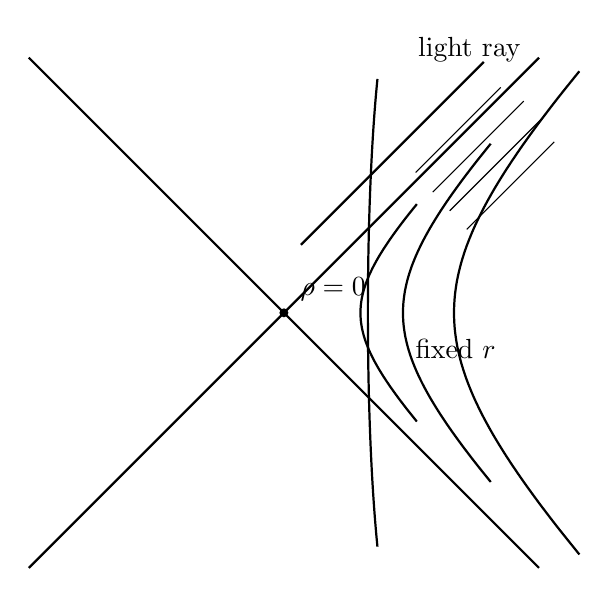
\begin{tikzpicture}[scale=1.08]
\draw[thick] (-3,-3) -- (3,3);
\draw[thick] (-3,3) -- (3,-3);

\fill (0,0) circle (1.5pt);

\draw[thick,domain=-1.15:1.15,smooth,variable=\u] plot ({0.9*cosh(\u)},{0.9*sinh(\u)});
\draw[thick,domain=-1.15:1.15,smooth,variable=\u] plot ({1.4*cosh(\u)},{1.4*sinh(\u)});
\draw[thick,domain=-1.15:1.15,smooth,variable=\u] plot ({2.0*cosh(\u)},{2.0*sinh(\u)});

\draw[thick] (1.10,-2.75) .. controls (0.95,-1.25) and (0.95,1.25) .. (1.10,2.75);

\draw[thick] (0.20,0.80) -- (2.35,2.95);

\draw[thin] (1.55,1.65) -- (2.55,2.65);
\draw[thin] (1.75,1.42) -- (2.82,2.49);
\draw[thin] (1.95,1.20) -- (3.05,2.30);
\draw[thin] (2.15,0.98) -- (3.18,2.01);

\node at (0.58,0.28) {\(\rho=0\)};
\node at (2.02,-0.42) {fixed \(r\)};
\node at (2.18,3.10) {light ray};
\end{tikzpicture}
\caption{A restrained redraw of the same near-horizon picture: null boundaries, several fixed-\(\rho\) trajectories outside the horizon, the distinguished point \(\rho=0\), and the extra fixed-\(r\) construction suggested by the board sketch.}
\end{figure}

This is where Susskind brings in Bob and Alice. Bob insists on staying outside the black hole, so near the horizon he follows one of the constant-\(\rho\) hyperbolae. That means Bob is accelerating. Alice lets go and falls freely, so in the near-horizon flat-space picture she follows an inertial line and crosses the horizon without encountering anything locally special.

The asymmetry is entirely observational. Bob never sees Alice cross the horizon; he sees her approach it more and more slowly, asymptotically flattening against it. Alice, on the other hand, crosses with no local drama and can still see Bob for a while by looking back along her past light cone. Susskind repeatedly insists that this should not be turned into a metaphysical puzzle about what ``really'' happens. The profitable question is always: what can each observer measure, see, or signal?

A stationary outside observer also has a physical asymmetry relative to the infalling one. To remain at fixed \(r\), Bob must accelerate, just as an observer standing on the ground accelerates relative to a freely falling frame. Nothing in the lecture suggests that Bob's description is wrong; rather, it is a description tied to accelerated worldlines that are causally barred from seeing through the horizon.

\section{Acceleration Horizons}

Susskind then steps back and says that none of this is uniquely about black holes. A uniformly accelerated observer in flat spacetime already has the same causal limitation. Such an observer sees a horizon beyond which signals never arrive and regards that boundary as the edge of the observable world. This is the acceleration horizon.

That remark is not a side comment. It is the conceptual payoff of the whole near-horizon analysis. The black-hole horizon, at least locally, is the gravitational version of the Rindler horizon of an accelerated observer. In this sense the lecture realizes Einstein's advice: to understand gravity, first understand acceleration.

\section{Temperature, Negative Specific Heat, and Evaporation}

After the break Susskind explicitly turns back to the previous lecture and puts on what he calls his ``thermodynamic hat.'' The guiding picture is the same as before: build a black hole by dropping in photons, each carrying one bit of information. That picture already suggested a relation between area and entropy. Now he wants to extract temperature and then use it to estimate the evaporation rate.

\paragraph{Temperature as the energy cost of one bit.}
Susskind pauses to define temperature in the operational way he wants to use it. Temperature is not taken as a primitive sensory notion; it is the minimum energy change required to increase the entropy by one unit, or in the language of the lecture, by one bit. For the black hole, one adds a photon whose wavelength is comparable to the hole size,
\begin{equation}
\lambda \sim R_s \sim \frac{2GM}{c^2}.
\end{equation}
The energy of one such photon is
\begin{equation}
E_\gamma \sim \frac{\hbar c}{\lambda}.
\end{equation}
Therefore, up to the order-one factors that the heuristic argument does not yet control,
\begin{equation}
T \sim \frac{\hbar c}{\lambda} \sim \frac{\hbar c^3}{GM}.
\end{equation}
This is the lecture's first-pass estimate: it is parametric, not exact.

Only after this scaling argument is on the board does Susskind quote the properly normalized Hawking temperature,
\begin{equation}
T_H = \frac{\hbar c^3}{8\pi GM}.
\end{equation}
The important qualitative lesson is already visible:
\begin{equation}
T_H \propto \frac{1}{M}.
\end{equation}
Large black holes are cold; small black holes are hot. The temperature is also manifestly quantum mechanical, since it vanishes with \(\hbar\).

\paragraph{Negative specific heat.}
This inverse dependence on \(M\) is exactly what makes black holes thermodynamically strange. Adding energy to an ordinary body usually raises its temperature. Adding energy to a black hole increases its mass and therefore lowers its temperature. A black hole has negative specific heat.

For a stellar-mass black hole, the lecture gives the order-of-magnitude estimate
\begin{equation}
T_H \sim 10^{-8}\ \mathrm{K}.
\end{equation}
That is much colder than the present cosmic microwave background temperature, about \(3\,\mathrm{K}\). A solar-mass black hole in today's universe is therefore not primarily an emitter; it is an absorber. It swallows surrounding radiation and grows colder as it grows more massive. If instead a black hole were hotter than its environment, it would radiate, lose mass, become hotter still, and run away in the opposite direction. Thermal equilibrium is unstable.

Susskind emphasizes that this instability is not peculiar to black holes alone. It is a familiar feature of gravitating systems more generally. A star that loses energy tends to contract and heat up, so gravity naturally produces systems with negative specific heat.

\paragraph{Evaporation in Planck units.}
To estimate the evaporation rate, Susskind now drops all the constants and works in Planck units,
\begin{equation}
c=\hbar=G=1.
\end{equation}
In these units energy is mass, so \(E=M\). The luminosity of any warm body is written, up to order-one factors, as
\begin{equation}
L=-\frac{dE}{dt}\sim A T^4,
\end{equation}
the Stefan--Boltzmann law. For a black hole,
\begin{equation}
A\sim R_s^2 \sim M^2,
\qquad
T\sim \frac{1}{R_s}\sim \frac{1}{M}.
\end{equation}
Substituting these scalings gives
\begin{equation}
-\frac{dM}{dt}\sim A T^4 \sim M^2\left(\frac{1}{M}\right)^4 = \frac{1}{M^2}.
\end{equation}
Equivalently,
\begin{equation}
M^2\frac{dM}{dt}\sim -1.
\end{equation}
Up to the ignored factor of \(3\), this is the statement
\begin{equation}
\frac{d(M^3)}{dt}\sim -1,
\end{equation}
so the evaporation time scales as
\begin{equation}
t_{\mathrm{evap}}\sim M^3.
\end{equation}

This is the main quantitative result of the second half. It immediately explains why macroscopic black holes live for absurdly long times. The lecture gives the corresponding solar-mass estimate by converting to Planck units:
\begin{equation}
M_\odot \sim 10^{38} M_{\mathrm{Planck}}
\qquad \Longrightarrow \qquad
t_{\mathrm{evap}}(M_\odot)\sim 10^{114} t_{\mathrm{Planck}}
\sim 10^{71}\ \mathrm{s}
\sim 10^{64}\ \mathrm{yr}.
\end{equation}
That is enormously longer than the present age of the universe. The later mountain-mass arithmetic in the lecture is too garbled to preserve confidently, but the scaling law \(t_{\mathrm{evap}}\sim M^3\) and the qualitative lesson are completely clear: very cold, very large black holes evaporate extremely slowly.

\paragraph{What this points to.}
Susskind does not yet try to explain the detailed mechanism of Hawking emission. Instead he treats temperature, entropy, and evaporation as clues. A system with entropy behaves, in this respect, like a fluid: the smooth macroscopic description is not the whole story. Entropy is evidence for hidden microscopic degrees of freedom. In that spirit, black-hole thermodynamics is read not as a finished theory but as a strong hint that ordinary classical gravity is an effective description hiding a deeper microstructure.

The lecture ends by sharpening the tension rather than resolving it. If black holes radiate and eventually give back information, then evaporation must somehow be reconciled with the horizon picture in which matter falls through. Susskind frames this not as a solved paradox but as the central problem still to be understood.

\section{Summary}

The lecture makes two claims and then supports both of them carefully. First, the horizon of a large black hole is locally uneventful: after an appropriate change of coordinates, the near-horizon Schwarzschild metric becomes the flat Minkowski metric in hyperbolic polar form,
\[
ds^2 = -\rho^2 d\omega^2 + d\rho^2.
\]
Second, black holes are thermodynamic objects: they have a quantum temperature inversely proportional to their mass, a negative specific heat, and an evaporation time that scales like \(M^3\) in Planck units.

What makes the lecture memorable is the order in which Susskind develops these points. He does not begin with polished final formulas. He begins with the apparent contradiction, detours into familiar coordinate systems, returns to the black hole only after the audience has the right model in mind, and then turns the resulting geometry into an operational story about observers, signals, and horizons. Only after the horizon has been made locally boring does he return to thermodynamics and let the real mystery reappear at a deeper level: if horizons are locally harmless but black holes have entropy and radiate, then gravity must be hiding more structure than the classical metric alone reveals.